
\documentclass[twoside,hidelinks]{article}

\usepackage{lipsum} % Package to generate dummy text throughout this template

\usepackage[sc]{mathpazo} % Use the Palatino font
\usepackage[T1]{fontenc} % Use 8-bit encoding that has 256 glyphs
\linespread{1.05} % Line spacing - Palatino needs more space between lines
\usepackage{microtype} % Slightly tweak font spacing for aesthetics

\usepackage{geometry} % Document margins
\usepackage{multicol} % Used for the two-column layout of the document
\usepackage{caption} % Custom captions under/above floats in tables or figures
\usepackage{booktabs} % Horizontal rules in tables
\usepackage{float} % Required for tables and figures in the multi-column environment - they need to be placed in specific locations with the [H] (e.g. \begin{table}[H])
\usepackage{hyperref} % For hyperlinks in the PDF
\usepackage{svg}

\usepackage{lettrine} % The lettrine is the first enlarged letter at the beginning of the text
\usepackage{paralist} % Used for the compactitem environment which makes bullet points with less space between them
\usepackage{amsmath}
\usepackage{abstract} % Allows abstract customization
\renewcommand{\abstractnamefont}{\normalfont\bfseries} % Set the "Abstract" text to bold
\renewcommand{\abstracttextfont}{\normalfont\small\itshape} % Set the abstract itself to small italic text

\usepackage{titlesec} % Allows customization of titles
\titleformat{\section}[block]{\large\scshape\centering}{\thesection.}{1em}{} % Change the look of the section titles
\titleformat{\subsection}[block]{\large}{\thesubsection.}{1em}{} % Change the look of the section titles
\usepackage{algorithm}% http://ctan.org/pkg/algorithm
\usepackage{algpseudocode}% http://ctan.org/pkg/algorithmicx

\algdef{SE}[FOR]{NoDoFor}{EndFor}[1]{\algorithmicfor\ #1}{\algorithmicend\ \algorithmicfor}%

\usepackage{fancyhdr} % Headers and footers
\pagestyle{fancy} % All pages have headers and footers
\fancyhead{} % Blank out the default header
\fancyfoot{} % Blank out the default footer
\fancyhead[C]{Master thesis $\bullet$ Panagiotis Chatzichristodoulou $\bullet$ 2015} % Custom header text
\fancyfoot[RO,LE]{\thepage} % Custom footer text

\usepackage{graphicx}
\graphicspath{ {pics/} }

%----------------------------------------------------------------------------------------
%	TITLE SECTION
%----------------------------------------------------------------------------------------

\title{\vspace{-15mm}\fontsize{24pt}{10pt}\selectfont\textbf{{Towards lifelong mapping in pointclouds}}} % Article title

\author{
\large
\normalsize \textbf{Supervisors} \\ 
\normalsize University of Maastricht \\ % Your institution
\normalsize \textit{Rico Mockel, Kurt Driessens} \\
\normalsize Dobots \\
\normalsize \textit{Anne Van Rossum} \\
\normalsize \textbf{Student} \\
\normalsize Panagiotis Chatzichristodoulou \\
\normalsize Student ID : I6076679
\vspace{-5mm}
}
\date{}

%----------------------------------------------------------------------------------------

\begin{document}

\maketitle % Insert title

\thispagestyle{fancy} % All pages have headers and footers

%----------------------------------------------------------------------------------------
%	ABSTRACT
%----------------------------------------------------------------------------------------

 
\begin{abstract}

\noindent Long term mapping is the natural conceptual extension to existing mapping methods. Mapping an area for long timeis a problem that if tackled efficiently will be a large step towards highly autonomous robots. As discussed in the literature lifelong mapping consists of two major subproblems. A compression, and a dynamic environment problem. The thesis discuses the application of non parametric Bayesian methods and how such tools can be directed to improve lifelong mapping capabilities of existing methods. A novel method of object clustering and matching is presented and its results are applied to an EKF SLAM algorithm; its strengths, weaknesses as well as future directions on how these tools could be extended to include dynamic environments are introduced.


\end{abstract}

%----------------------------------------------------------------------------------------
%	ARTICLE CONTENTS
%----------------------------------------------------------------------------------------
\newpage
\thispagestyle{empty}
 
\tableofcontents

\listoffigures
 
\listoftables
 
\newpage


\section{Introduction}


Simultaneous localization and mapping is one of the fundamental problems of autonomous systems\cite{probRobs}. In order for a robot to be considered truly autonomous, it must have the ability to enter an area and infer its structure. To that direction, a lot of effort has been put in algorithms that are able to map static environments. With solutions like EKF-SLAM\cite{ekf}, FastSlam\cite{slam} and GraphSLAM\cite{graph} robots are now able to efficiently map static environments. 
The logical extention to methods that can map  static environments is methods that remove this restriction. The idea of lifelong robot learning is not new and has been introduced as a general concept to the literature by Sebastian Thrun~\cite{liflonglearning}. Konolige et al.\cite{lifelongmaps} specifically focus on lifelong learning in mapping and the utility such methods would have.  In the PhD thesis of Walcott~\cite{aishalong} long term mapping is decomposed to 4 basic subproblems:
\begin{itemize}
	\item{Continuously incorporate new information.}
	\item{Address the problem of tractability for growing DPG}
	\item{Representation of the environment should include the history of the map as changes occur	with the passage of time.}
	\item{Detect changes and update the map online}
\end{itemize}

The first two problems can be though of as compression problems as the map increases over time whereas the latter ones can be though of as dynamic environment problems. Methods of tackling those problems vary according to what sensors a robot uses to perform the mapping. In this project the focus will be directed in methods that use RGBD devices to perform SLAM like Microsoft's Kinect.

Since its introduction in 2010 Microsoft Kinect\cite{kinect} has revolutionized RGBD devices with its low price range and high quality sensors. It came as no surprise that research in point clouds, the representation system of Kinect sensor readings, has increased since. Many libraries that enable the user to perform tasks from feature extraction to plane segmentation\cite{pcl} in pointclouds are currently available. In the field of robotics, many teams are using the Kinect sensors to perform simultaneous localization and mapping\cite{rtabmap}. The goal of this thesis is to introduce a novel approach to tackle the compression problem of long term mapping methods that use the Kinect device by using Bayesian non parametric methods.

Dirichlet processes and Dirichlet process mixture models \cite{nonParam} are the cornerstone of Bayesian non parametric statistics. The strength of those models lies in the fact that they allow the model's mixture components to grow as much as needed so as to best fit the data. The dynamic number of components in combination with the highly resilient priors leads to very flexible models that can be used in a very large area of applications from topic modeling\cite{LDA} to speaker diarization\cite{speakerDiar}. 

The main motivation behind this project is to use such methods as a means of compressing the information provided by the environment. In that direction, finding a way to robustly cluster a point cloud into semantically sound "chunks" of structure seems a reasonable starting point. This leads to the direction of object based SLAM, which is a domain where objects are used as reference points to perform the mapping.

In this paper, an EKF SLAM method that takes point clouds as input will be implemented. More specifically, a landmark detection layer using the clouds as input will be added; its results will then be empirically tested as well as its ability to optimally compress the data a point cloud. Its strengths and weaknesses will be presented and analysed; furthermore, directions on how the method could be extended to tackle the first two subproblems of Walcott's thesis will be given in the discussion.

The rest of the paper is structured as follows. Section \ref{sec:literature} will present relevant literature review, Section~\ref{sec:theory} will introduce the theories behind the model, Section~\ref{sec:model} will define the model, Section ~\ref{sec:results} will show experimental results of the method. Finally, Section ~\ref{sec:discussion} will end up with a discussion on the methods strengths and weaknesses.

%------------------------------------------------
 
\section{Literature review}
\label{sec:literature}

Related research will be focused on 4 general sub fields of related literature.
\begin{itemize}
	\item Object based SLAM or semantic slam
	\item Point Cloud Object segmentation
	\item Non-parametric clustering methods
	\item The correspondence problem in SLAM
\end{itemize}

More specifically, object based SLAM is crucial due to the nature of the input the method at hand has. Since point clouds are used as input and from such input object representations must be extracted, methods that use such approaches to perform SLAM are then needed. The second part of the research is focused on point cloud representations. This part of the research is mostly focused on what features or meta-features need to be taken into account so that the reduced representation is solid. The third part of the research is focused on non-parametric Bayesian methods and the clustering tools they provide. Such tools are important as they can be used to provide new approaches to object segmentation within a point cloud. Finally, research is focused on the correspondence problem in SLAM. As one of the fundamental problems that need to be solved in order to have robust SLAM algorithms, it is imperative the correspondence problem be solved efficiently. In that extent and due to the unique representation of our objects, a novel approach that takes elements from other techniques in the correspondence between objects in a SLAM problem is given.

\subsection{Object based SLAM}
Object based SLAM or semantic slam methods proposed in the literature focus at domain specific solutions of particular problems. Salas-Moreno et al~\cite{slam++} define a method of performing object based slam for specific objects. The objects are identified by camera that is on top of the robot. By having a model of pretrained objects, SLAM can be performed on environments the robot knows what objects to expect. The disadvantage of that method is that object models have be to be well defined and there is a small number of such objects. 
Castle et al. use object recognition to perform object based SLAM with the use of a hand-held cameras. Selvatici et al~\cite{objslam} use a similar approach while exploiting structural information such as object height and position within the room. That way a couch that is a large object situated in floor level is easier to be recognized.
Choudhary et al.~\cite{objectpointslam} use point clouds and an object database to match objects currently seen with known objects within their database. They use omnimaper~\cite{omnimaper} as their mapping method and as a representation a combination of the downsampled  voxel grids with additional normal and curvature information.  Finally, all their operations are done in the non-planar components of the point cloud.
Jensfelt et al~\cite{objslam} present an object based approach to SLAM where the robot can manipulate the objects of the map. They use camera pictures as input and receptive Field Histogram as the method to abstract the camera input and extract features for their object matching algorithm. Their approach is proposed as a solution to a service robot scenario.
MonoSLAM~\cite{monoslam} introduces a method of performing slam using a monocular camera. 

What all the previous methods have in common is that they approach the problem of object based slam as a classification task. Objects need to be semantically understood before they are processed. The approach introduced in this paper considers the environment to be a collection of chunks. So having specific enough environment descriptors should lead to the robot being able to operate in a label free environment. This would remove the need of having to classify objects but would also increase the time it takes to extract features from the environment as features are the base of the unsupervised object discovery.
Seongyong Koo et al.~\cite{objectDisc} introduce a method of unsupervised object individuation from RGB-D image sequences. They cluster their initial cloud into candidate objects using Eucledian clustering and proceed to extract features like the Euclidian distance(L2) and the Kullback-Leibler distance between point cloud objects. They use IMFT to solve their tracking problem.

\subsection{Point Cloud Object segmentation}

Research towards object segmentation in point clouds is focusing on calculating meta information regarding the points and applying some heuristic function to see if the points could belong in the same segment of the cloud. Trevor et al.~\cite{pointSeg} take positional information, Euclidean distances and the normal of points to as input to their heuristic and output segments that are part of the same object. PCL library~\cite{pcl} introduces methods like Euclidean clustering and conditional Euclidean clustering that use a number of heuristics that take normal as well as curvature information to extract segments in the point cloud that represent objects. Furthermore, a there is a lot of resarch on segmentation of point clouds in scenes, the emphasis is usually on extracting geometric primitives~\cite{planarSeg},~\cite{planarSeg2} using cues like normals and curvature. Rabbani et al~\cite{segOverview} introduce a new method of object segmentation using KNN as their base algorithm. They also present a very informative literature review along with the strengths and weaknesses of existing methods. Finally Triebel et al.~\cite{smartSeg} introduce a general clustering framework that does not rely on plane segmentation. Instead of segmenting the plane by using classical approaches like RANSAC or MLASAC they introduce a framework where they make no assumptions regarding plane data. 

\subsection{Non Parametric Bayesian methods}

Bayesian non-parametric methods are the cornerstone of Bayesian statistics. In this project the focus was directed towards the clustering methods that are being introduced by those tools. Radford M. Neal~\cite{bayes:neal} with his paper regarding MCMC methods for Dirichlet process mixture models made the definitive step towards Dirichlet process mixture models(DPMM's) receiving a lot of attention. Since then, a variety of approaches for inference on such models has been introduced with Statistical inference and MCMC methods, and Variational inference being two prominent ones. Variational inference for DPMM's was introduced by Jordan et al.~\cite{bayes:jordan} and it introduces deterministic tools to perform inference and approximate the posterior distribution and marginals of a dataset. Both methods have strengths and weaknesses and many tools have been established by using the two approaches as their base. Blei et al.~\cite{LDA} introduced LDA as a method to perform topic modelling. Teh et al~\cite{bayes:hier} introduce a hierarchy on the inference process by introducing the Hierarchical Dirichlet process. Particle filter approaches have also been established. Doucet et al.~\cite{bayes:smc} introduce Sequential Monte Carlo as a fast way to approximate inference. Inference on Dirichlet process mixtures is a very active research field and covering it is beyond the scope of this report. In this project SMC samplers where used due to their robustness as well as their inherent extensiveness. A detailed description on the mechanisms of sequential samplers will be given in the theory section.

\subsection{Correspondence}

In its general definition, the correspondence problem refers to the problem of ascertaining which parts of one image correspond to which parts of another image, where differences are due to movement of the camera, the elapse of time, and/or movement of objects in the photos. Under the semantic SLAM context, it refers to the problem of identifying objects as objects that have been encountered before during the mapping process. Towards that direction Cree et al.~\cite{corresp:first} create a histogram of line segments of each landmark and compute their root mean square error. They then proceed to calculate their RGB signature to calculate the distance between different landmarks. Low et al.~\cite{corres:sec} match Scale Invariant Feature Transform (SIFT) features, an approach which transforms image data into scale-invariant coordinates relative to local features. Lamon et al~\cite{corres:three} store a database of fingerprints which indicate the location in the robot's environment. The features are ordered and stored at a database at as they appear in the robot's immediate surroundings. A new fingerprint is computed for each new view and matched against existing ones. Finally, in Seghal et al.~\cite{corres:four} an extension of SIFT descriptors to 3D data and point clouds is given.

The approach presented in this paper takes an input similar to~\cite{objectDisc} as parts of the point cloud are being clustered a mixture of distributions. The features that are used for the cloud representation are an extension of the features presented in~\cite{smcddp} with the addition of angle information present in the points of the cloud. Since the operations are now done on cluster level, the distances among clusters can be then represented as distances between distributions and there has been extensive search on that field. Distances like Hellinger, KL divergence, Euclidian, Mahalanobis can all be taken into account when performing the object matching. The robustness of the method can also be increased by using tracking methods like IMFT. The novelty lies in its completely probabilistic mechanism as the clustering is done by using SMC to the augmented feature space. Using distributions as a means of representing objects within the point cloud is a form of compression as objects are represented by a distribution which is smaller in size and easier to maintain and expand. Finally, instead of using heuristics, the distribution correspondence is done through a trained random forest model.
  


%------------------------------------------------

\section{Theory background}
\label{sec:theory}

A basic background of GPU

\subsection{Generalized Polya's Urn}
Dirichlet process priors have been widely used in the literature as non parametric Bayesian tools to estimate the number of clusters in the data~\cite{antoniak}. Dependent dirichlet processes extend those priors by allowing the clusters in the data to vary with some covariance over time. Dependent Dirichlet processes(DDP) remove the restriction of exchangeable data and introduce dependencies which can be temporal, positional etc. The DDPs are a natural extension of the DP's in domains where data cannot be considered exchangeable and have dependencies that cannot be disregarded. They where introduced by MacEachern~\cite{theory:ddp} and have been widely used since. The main motivation behind using such methods is the immediate extension they provide to dynamic environments. 

A DDP also known as Generalized Polya Urn~\cite{caron} and has the property of randomly deleting partitions of clusters on every iteration. That way, it can cope with the variance of the data. In the current project, the $n_th$ datapoint at time $t$,$x_{t,n}$ has an assignment $c_{t,n}$ at cluster $k \in \{1,2,..., K\} $. The size of cluster $k$ at time $t$ is defined as $s_t^k$. The GPU of this model at time $t$ can now be defined as:



\begin{algorithm}
  \caption{GPU}\label{GPU}
  \begin{algorithmic}[1]
    \Procedure{GPU}{$pointCloud, t$}

      \For{\texttt{$k = 1,...K_{t-1,N_{t-1}}$}}
	      \State Draw $\Delta s_{t-1}^k \sim Binom(s_{t-1,N_{t-1}}^k, \rho) $ \Comment{Number of elements to delete}
	      \State Set $s_{t,0}^{k} = s_{t-1,N_{t-1}}^{k} -\Delta s_{t-1}^k$
      \EndFor
      \For{\texttt{$n = 1,...N_t$}}
      	    \State Draw $c_{t,n} \sim Cat( \frac{ s_{t,n-1}^{1} }{\alpha + \sum_k s_{t,n-1}^{k} }, \frac{ s_{t,n-1}^{K_{t,n-1}} }{\alpha + \sum_k s_{t,n-1}^{k} } , \frac{ \alpha}{\alpha + \sum_k s_{t,n-1}^{k} }) $
      	    \State If $c_{t,n} \leq K_{t,n-1}\ set:\ s_{t,n}^{c_t,n} = s_{t,n-1}^{c_t,n} + 1 , K_{t,n} = K_{t,n-1}$
      	    \State If $c_{t,n} > K_{t,n-1}\ set:\ s_{t,n}^{c_t,n} = 1 , K_{t,n} = K_{t,n-1} + 1$
      \EndFor
    \EndProcedure
  \end{algorithmic}
\end{algorithm}


Where Cat is a categorical distribution, Bin is the binomial distribution, $\alpha$ is the DP concentration parameter and $\rho$ is the deletion parameter of the GPU. This Generative Polya Urn distribution also has the shorthand notation GPU($\alpha,\rho$)

This process can be though of in the terms of a general Chinese restaurant process as shown in Fig.~\ref{generalPolya}. At time $t$ (a), suppose there are customers seating at several tables in the restaurant. Each customer has to decide if he/she will remain at table with probability $p$ or leave the restaurant with probability $1-p$. Once all the customers make their decisions they leave the restaurant or remain seated (b). Each table occupied is moved according to the number of customers still seating in that table (c). A new customer then enters the table and either chooses to sit on one of the existing tables (e) or choose a new with probability proportional to the strength parameter $\alpha$ of the model (f).

\begin{figure}[h!]
  \centering
    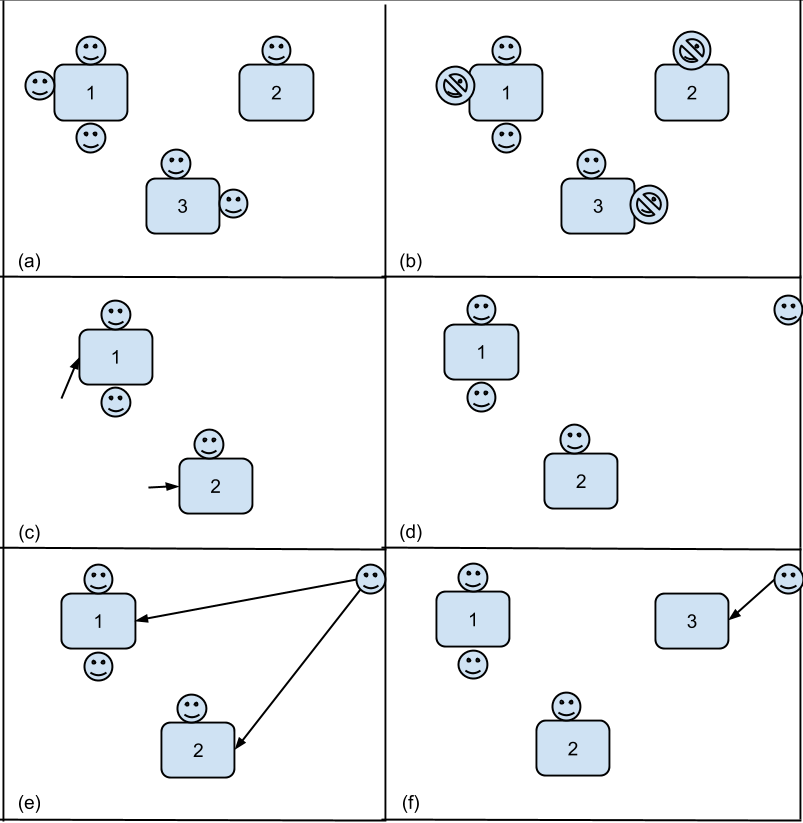
\includegraphics[width=.65\textwidth]{generalPolya}
    \caption{Generalised Polya Urn as presented in CRP.}
  \label{generalPolya}
\end{figure}

\section{Model definition}
\label{sec:model}

\subsection{General pipeline}
Now that the data distribution and sampler are defined, the model that takes as input point clouds from a Kinect sensor mounted on a robot and outputs the most probable landmarks given the input and the previous landmarks can be presented. Fig.~\ref{pipeline} depicts the general workflow of what happens during the observation step of SLAM. The SLAM node-- requires landmark information, and the landmark pipeline outputs the most probable landmarks given the current database of landmarks and the current observations. If needed landmarks added to the database and the landmark ids are given to back to the SLAM node.


\begin{figure}
\begin{tabular}{cc}
  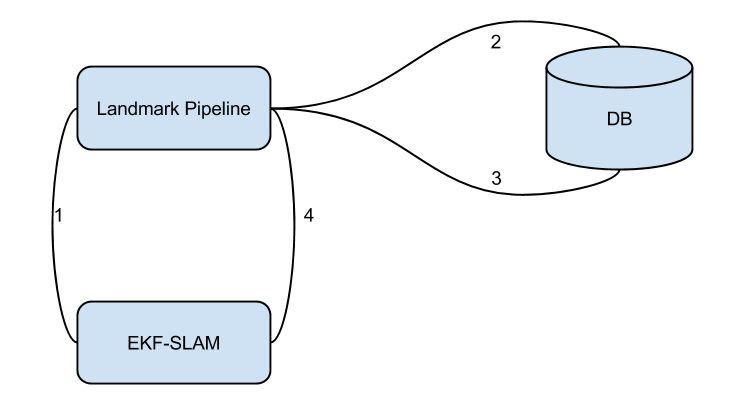
\includegraphics[width=65mm]{workflowGen} &    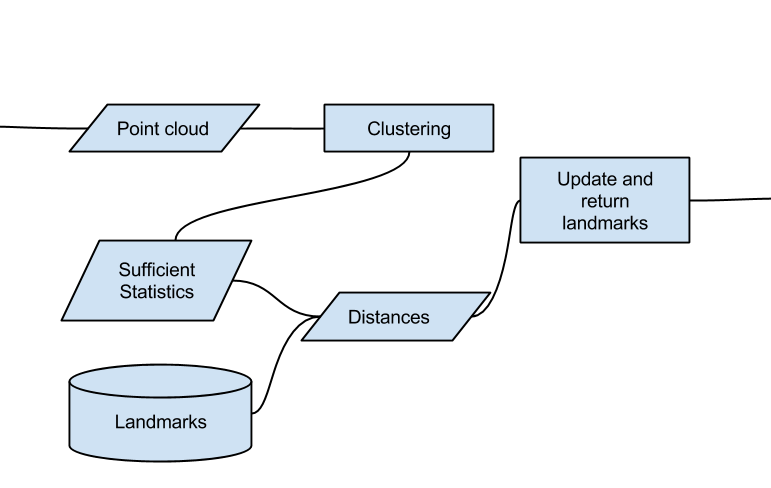
\includegraphics[width=65mm]{workflowSpec} \\
(a) General pipeline & (b) Landmark pipeline \\[6pt]
\end{tabular}
\caption{General landmark update pipeline}
\label{pipeline}
\end{figure}

The model introduces a Pipeline in the layer of landmark detection of the EKF-SLAM algorithm. All the operations from feature extraction to clustering and object matching will be performed at that layer. More specifically the pseudo-code for the method is the following:

\begin{algorithm}
  \caption{Landmark Layer}\label{euclid}
  \begin{algorithmic}[1]
    \Procedure{getLandmarkIds}{$pointCloud, timepoint, existingLandmarks$}\Comment{Post transformation}
      \State $initialize(landMarkIds)$ \Comment{Initialize empty list}
      \State $pointCloudReduced \gets extractMetaFeatures(pointCloud)$ \Comment{Cloud preprocessing}
      \State $features \gets extractMetaFeatures(pointCloudReduced)$
      \State $landmarks \gets cluster(features)$  \Comment{Cluster using features}

      \For{\texttt{$landmarks$ as $landmark$}}
	      \State $ (probability, landId) \gets getBestLandmarkCorrespondence(landmark, existingLandmarks) $
			\If{$probability >threshold$}
			   \State $ addLandmarks(landMarkIds, landId)$\Comment{Return known landmark}
			\Else 
			   \State $ newLandID \gets addLandmarkDB(landmarkDB, landmark)$ \Comment{Add get new id}
			   \State $addLandmarks(newLandID)$ \Comment{Add landmark}	   
			\EndIf
      \EndFor
      \State \textbf{return} $ landMarkIds$\Comment{Return added landmark}
    \EndProcedure
  \end{algorithmic}
\end{algorithm}


This top level description has a lot of implied steps so a line by line description will be provided:

\textbf{Method input:} The method takes as input a point cloud. The post transformation comment has to do with the fact that the 
cloud expected is the one after all the frame transformations are done in the tf layer of the robot.

\textbf{Lines 3-4:} Feature extraction is done through the pcl~\cite{pcl} library. An initial point cloud reduction is mandatory to increase the speed of the process. A voxel grid is used to reduce the dataset size. A leaf size of approximately 4cm produces a good tradeoff between precision and speed. The object representation approach is similar to~\cite{objectpointslam}. Instead of using the CSHOT descriptor, pcl's fpfh~\cite{fpfh} is being used. Fast point feature histogram(fpfh) represents an angular signature between a point and its neighbors. In that way we end up with a 23 dimensional angular signature of information between a point and its neighbors. Since the information are given in the form of a histogram, classical statistic solutions regarding the distances between angular signatures can be taken into account. In our solution EMD,Hellinger,and KL divergence are being computed in the pipeline. Color information is being encoded with an approach similar to ~\cite{smcddp}. The colour spectrum is discretized and what is extracted is the count of different colour signatures between a point and its k nearest neighbors. Finally positional information is also given as input to the algorithm. The pipeline is presented in figure Fig.~\ref{pcl:mod}. What the algorithm outputs is then a vector of $ \textbf{x} = (x_s, x_c, x_a) $ where $s$ represents a 3x1 vector of space information, $c$ a 27x1 vector of colour information and $a$ angular information whose dimensionality depends on the distances computed(in our case 3x1). It must be noted that pcl offers a multi threading operation on the point feature histogram extraction. This feature is important since it greatly reduces(6-8 times) the speed of an operation applied on every point of the cloud and that makes the histogram extraction significantly faster.

\begin{figure}[h!]
  \caption{Point cloud modification pipeline.}
  \centering
    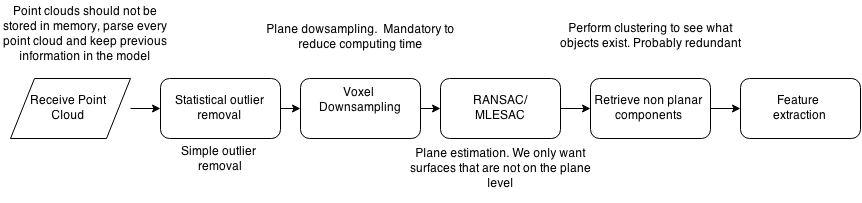
\includegraphics[width=1\textwidth]{Basic}
  \label{pcl:mod}
\end{figure}

\textbf{Lines 5:} The clustering takes place in this line. The input of the method is the feature vector for every data point which is calculated in the previous steps. An SMC sampler is used as was presented in the theory section. 

\textbf{Lines 6-12:} The correspondence of the previous landmarks to current ones happens in theses lines. Since the landmarks are distributions, statistical distances can be taken to perform the matching. The distances are then discretized and are being given as input to the getBestLandmarkCorrespondence. The getBestLandmarkCorrespondence function is a random forest implementation. An offline model has been trained to recognize correlation between those distances and landmark detection. This approach is similar to~\cite{objectDisc}. It must be noted that the method depends on the training to be general enough so a good initial data set is mandatory. The random forest outputs the probability of a landmark having been encountered before; if the probability is high enough, it is being added to the landmarks list to be send for update in the EKF, otherwise a new landmark is added and its ID is then updated to the list.

\textbf{Lines 15:} The algorithm returns the list of the most probable landmarks the robot encounters in this current time.


Now that the general pipeline is defined, the data distribution as well as the sampler can be introduced.


\subsection{The data distribution}

Each point $x$ in the input consists of a tuple $x =(x^s, x^a, x^c ) $ where superscript $s$ represents spatial information, $a$ angle information, and $c$ colour information. The method those features are extracted is explained in lines 3 and 4 in the general pipeline. For the purpose of this project each part of the cloud was represented by vector of length 32 with the first three elements representing the space information, elements 4-6 angle information, and the rest colour information.

The object model is a mixture of distributions over the data with each object beign modeled as D($\theta_t^k$) where $\theta$ represents the parameters of object $k$ at time $t$. More specifically, each set \textbf{x} with $n$ datapoints at time $t$ is distributed as:
$$ x_{t,n} \sim D(\theta_t^k) = Normal(x_{t,n}^s| \mu_t, \Sigma_t) Mult(x_{t,n}^c | \delta_t) Exp(x_{t,n}^a | \lambda_t) $$

Where Normal is a three dimensional Gaussian distribution with mean $\mu$ and covariance $\Sigma$ representing the positional distribution of the data; Mult is a Categorical multinomial distribution with parameter vector $\delta$ representing weigths the colour distribution and Exp is an exponential with shape parameter $\lambda$ representing the angle distribution of the data within the cluster. The exponential distribution was chosen to model angular information after empiric evaluation showed that it would be a good fit for the angle signature distribution of the data. A typical angle signature distribution is shown in.~\ref{pcl:kl}. For this graph data points from various point clouds where taken and passed through the pipeline analysed in lines 3-4. The data were then plotted, and the figure shows what the aggregated angle distribution between neighbor datapoints is. Since there is a clear exponential trend, the exponential distribution was chosen to model it. A gamma distribution is also a nice fit for the data, but due to time constrains, only one modeling    distribution was explored.

\begin{figure}[h!]
  \centering
    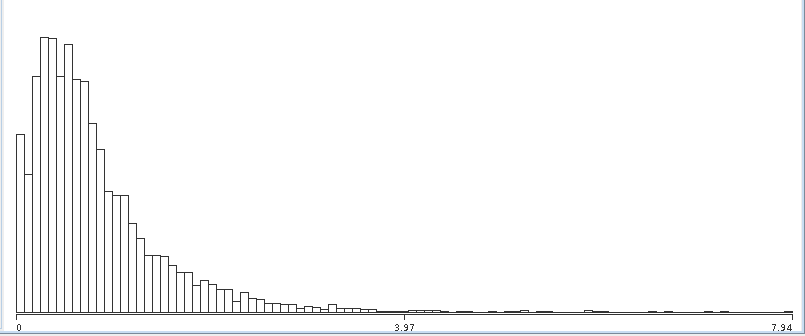
\includegraphics[width=.5\textwidth]{Kullback-Leibler}
    \caption{Exponential trend in KL distances.}
  \label{pcl:kl}
\end{figure}


Now that the distribution of the objects is defined, the progression of the sufficient statistics at time $t$ given $t-1$ given by:

$\theta_t^k | \theta_{t-1}^k \sim
\begin{cases} T (\theta_{t-1}^k) &\mbox{if } k \leq K_{t-1} \\
G_0 & \mbox{if } k > K_{t-1}. \end{cases}$

Where $T$ represents the transition kernel of the data given the previous state in the model. The case $ k > K_{t-1} $ represents the creation of a new cluster and $G_0$ is the base distribution of the DDP. In our case, the conjugate priors of the distributions of the data were chosen to model the base distribution. Therefore, $G_0$ is defined as:

$$ G_0(\theta_t^k)  = NiW( \mu_t^k, \Sigma_t^k | \kappa_0, \mu_0, \nu_0, \Lambda_0 ) Dir(\delta_t^k | q_0) Gam( \lambda_t^k | \alpha_0, \beta_0) $$

Where NiW is a Normal inverse Wishart distribution, Dir denotes a Dirichlet distribution, and Gam the Gamma distribution. $ \kappa_0, \mu_0, \nu_0, \Lambda_0, q_0,\alpha_0$ and $\beta_0$ are predefined parameters of the model. The generative process for the Dependent Dirichlet mixture model can be written for each timestep $t$ as:

\noindent\makebox[\linewidth]{\rule{\textwidth}{0.4pt}}
\begin{enumerate}
	\item Draw  $c_t$ $\sim$ $GPU(\alpha, \rho) $
	\item $\forall$  k draw: $ \theta_t^k | \theta_{t-1}^k \sim
	\begin{cases} T (\theta_{t-1}^k) &\mbox{if } k \leq K_{t-1} \\
	G_0 & \mbox{if } k > K_{t-1}. \end{cases}$
	\item $\forall$  point $n$ draw $ x_{t,n} \sim F(\theta_t^{c_t,n})$
\end{enumerate}
\noindent\makebox[\linewidth]{\rule{\textwidth}{0.4pt}}
Given the theory in \cite{caron}, the transition Kernel must satistfy:

$$ \int G_0(\theta_k) T(\theta_t^k | \theta_{t-1}^k) d\theta_{t-1}^k =  G_0(\theta_k) $$

The equation means that the invariant distribution must equal its base distribution. A typical way of meeting this restriction and forcing the sampler to converge to the original target density\cite{smc:theory} is to introduce a set of M auxiliary variables \textbf{z} such that:

$$ P(\theta_t^k | \theta_{t-1}^k) =  \int P(\theta_t^k | z_{t}^k)   P(z_t^k| \theta_{t-1}^k) dz_t^k $$

The transition kernel of the model can now be sampled by using the following formula

$\theta_t^k \sim T(\theta_{t-1}^k) = T_2 \circ T_1(\theta_{t-1}^k)$ where:
\begin{equation} \label{eq1}
\begin{split}
z_t^k  & \sim T_1(\theta_{t-1}^k)\\
 & = Normal(\mu_{t-1}, \Sigma_{t-1}) Mult( \delta_{t-1}) Exp( \lambda_{t-1})
\end{split}
\end{equation}

\begin{equation}
\begin{split}
\mu_t, \Sigma_t, \delta_t,  \lambda_t & \sim T_2(z_t^k)\\
 & = NiW( \kappa_0, \mu_0, \nu_0, \Lambda_0 ) Dir(q_0) Gam(\alpha_0, \beta_0) 
\end{split}
\end{equation}

where $\mu_t, \Sigma_t, \delta_t,  \lambda_t$  are posterior parameters given the auxiliary variables $z$.

\subsection{Sequential monte carlo sampler}

Sequential monte carlo samplers for Dirichlet process mixture models where introduced by Doucet et al~\cite{doucet} and serve as fast alternative to MCMC and VI methods of performing posterior inference. SMC samplers have known strengths and weaknesses and are a good fit for the problem at hand, as their main theoretical disadvantage which is the particle degradation cannot occur in a time horizon of 1 that the sampler is being used. We can now define the SMC sampler that will be used to perform inference on our model as follows:

\begin{algorithm}[h]
  \caption{SMC for DDPM}\label{SMC}
  \begin{algorithmic}[1]
	\State \textbf{Input:} Points \{$x_{1,1:N_t}, ..x_{T,1:N_t}$\}with extracted features
	\State \textbf{Output:} Clusters representing of the data
	\For{$t = 1,...T$} 
			\For{$ l = 1,...L$} 
							\For{$ iter = 1,...S$} 
								\State Sample $(c_t)^{(l)} \sim Q_1$  
								\State Sample $(\theta^k ) \sim Q_2$
						    \EndFor		
		    \EndFor
		    \For{$ k = 1,...K$} 
			   \State Sample $\Delta s_{t-1}^k \sim Binom( (s_{t-1,N_{t-1}}^k)^{(l)}, \rho) $ 
		       \State Set $s_{t,0}^{k} = s_{t-1,N_{t-1}}^{k} -\Delta s_{t-1}^k$
   		       \State Sample $( (z_{t+1}^k)^{(l)} ) \sim T_1((\theta_t^k))^{(l)} $
		    \EndFor
		 	\State compute particle weights $w_t^l$
    \EndFor
    \State Normalize and resample weights
  \end{algorithmic}
\end{algorithm}

\subsubsection{Gibbs updates}
The proposal distribution $Q_1$ is the probability of an assignment $c_{t,n}$ given cluster sizes, parameters and concentration $\alpha$. Formally $Q_1$ can be written as:
\begin{equation} \label{Gibbs}
 Q_1(c_{t,n} | s_{t,n}^k, \theta_t^k, \alpha) \propto Cat( s_{t,n}^1,...s_{t,n}^K, \alpha ) \times
 	\begin{cases} 
 	F(x_{t,n} | \theta_t^{c_t} )  &\mbox{if } k \leq K_{t-1} \\
 	\int P(x_{t,n} | \theta_t )G_0(\theta) d\theta & \mbox{if } k > K_{t-1}. \end{cases}
\end{equation}
Where $c_{t,n}$ represents cluster $c$ of point $n$ at time $t$, $s$ represents cluster sizes. The integral represents the posterior predictive distribution of the cluster times the base distribution with the parameters integrated out. A review of the literature helps understand how the posterior predictive formula is derived. More specifically, the analytic expression of the integral is:


\begin{equation} \label{Q1}
	\begin{split}
		 	\int P(x_{t,n} | \theta_t )G_0(\theta) d\theta =
		 	\int Normal(x_{t,n}^s| \mu_t, \Sigma_t) Mult(x_{t,n}^c | \delta_t) Exp(x_{t,n}^a | \lambda_t) \times  \\ NiW( \mu_t, \Sigma_t | \kappa_0, \mu_0, \nu_0, \Lambda_0 ) Dir(\delta_t | q_0) Gam( \lambda_t | \alpha_0, \beta_0)  d\theta  \\
			= \int Normal(x_{t,n}^s| \mu_t, \Sigma_t) \times NiW( \mu_t, \Sigma_t | \kappa_0, \mu_0, \nu_0, \Lambda_0 )\\
			 Mult(x_{t,n}^c | \delta_t) \times Dir(\delta_t | q_0) \\
			 Exp(x_{t,n}^a | \lambda_t) \times  \times Gam( \lambda_t | \alpha_0, \beta_0)  d\theta  \\
		 	= t_{\nu_0-1}( x_{t,n}^s | \mu_0, \frac{\Lambda_0(\kappa_0+1)}{\kappa_0(\nu_0-1)}) \times \prod_{j=1}^V \frac{\Gamma(x_{t,n}^c)}{\Gamma(q_0)} \times \\ \frac{\Gamma(\sum_{j=1}^V q_0)}{\Gamma(\sum_{j=1}^V x_{t,n}^c)} \times Lomax(\alpha_0 + s_{t,n}^c, \beta_0 \sum_{j=1}^V x_{t,n}^c)
 	\end{split}
\end{equation}

Where $t$ represents student's t-distribution with $\nu$ degrees of freedom, Lomax represents Lomax distribution with shape and scale, $\alpha$ and $\beta$ repsectively and the rest represent a Dirichlet-Multinomial(aka DirMul) distribution. The formulas of the posterior predictive distributions can be found in the literature with \cite{compendium} being a good example. 

The conjugacy of the base and prior distribution allows for an easy sampling formula for proposal distribution $Q_2$ which is of the form: 


\begin{equation} \label{Q_2}
\begin{split}
Q_2(\theta_t^k | \theta_{t-1}^k , x_t^k, z_t^k) \propto F( x_t^k | \theta_k) \times T_2(\theta_t^k | z_t^k) \\
= NiW( \mu_t^k, \Sigma_t^k | \kappa_n, \mu_n, \nu_n, \Lambda_n ) Dir(\delta_t^k | q_n) Gam(\lambda_t^k | \alpha_n, \beta_n)
\end{split}
\end{equation}

With:

\begin{equation} \label{udpates}
\begin{split}
\kappa_n = \kappa_0 + N \\
\nu_n = \nu_0 + N \\
\mu_n = \frac{\kappa_0}{\kappa_0 + N} \mu_0 +  \frac{N}{\kappa_0 + N} \overline{x}^s\\
\Lambda_n = \Lambda_0 + s_{x}^s\\
q_N = q_0 +  \sum_n x_i^c\\
\alpha_n = \alpha_0 +  N\\
\beta_n = \beta_0 +  \sum^n x_i^a\\
\end{split}
\end{equation}


Where $\overline{x}$ defines the sample mean for the elements assigned at cluster $c$, $s_{x}$ the sample variance and $N$ denotes the number of observations. The formulas for the updates can be found at the literature of cojugate priors with\cite{conjugate} being a good example.

\subsubsection{Weight updates}

The only thing left to explicitly define the sampler in its whole is the weight update step. More specifically, on every time step $t$ the weight of particle $l$ is calculated as:

\begin{equation}
w_t^{(l)} = \frac {P(c_t^{(l)} , \theta_t^{(l)}, x_t| 	\theta_{t-1} )}{P(c_t^{(l)} , \theta_t^{(l)}| 	\theta_{t-1} )}
\end{equation}

Using bayes rule, the numerator can be written as:

\begin{equation}
	P(x_t , | c_t^{(l)} , \theta_t^{(l)} \theta_{t-1} ) \times P(c_t^{(l)} , \theta_t^{(l)}|  \theta_{t-1} )
\end{equation}

Which can be calculated using equations $Q_2$ and $Q_1$ for the first and second part respectively. After the particle weights are normalized particles are drawn with probability proportional to their weights.



\subsection{Complexity}

The complexity can be decomposed into three major parts. The cloud downsampling, the clustering and the decision making.

\textbf{Downsampling}: The complexity of the cloud can be reduced to the complexity of its components. This means that the decomposed complexity is defined as follows:
$$O(filter) = O(Vox\ Downsampling + Stat\ Removal + RANSAC+ FPFH + Color\ estimation) $$

Voxel downsampling searches for neighbors within a distance defined by the user and keeps an average value that equally represents the cloud. Since the operation involves searching for neighbors of a point, and under the assumption that search operations take $O(log\ n)$ time where N is the number of points within the cloud, the complexity of voxelGrid downsampling is $O(k log n)$ where $k$ defines the number of neighbors and $n$ the number of points in the cloud.
Statistial outlier removal searches for k nearest neigbhors and removes those whose deviation is passed a certain threshold. Given that search operations take $O(log\ n)$, for k neighbors, the complexity is $O(k\ log\ n)$.
A high amount of research has been done regarding the optimal complexity of RANSAC~\cite{RANSAC}. RANSAC has a complexity of $ O(k(t_M)+ m_s*N)$ where k is the maximum amount of iterations defined by the user, $m_s$ the average number of models per sample $N$ the number of data points and $t_M$ the time needed to draw a sample. The time variance also depends on the hardware.
FPFH has a complexity of $O(nk)$ as given in~\cite{fpfh}.
Finally, for the operation of color estimation, the k nearest neighbors are chosen and some constant operation is performed on them. The complexity here is similar to Statistical outlier removal since operations after the search take a constant time $O(k\ log\ n)$ where $k$ is the number of neighbors, $n$ the number of points. 

The downsampling pipeline has then a complexity of 
\begin{equation} \label{Q_filt}
O(filter) = O(k_{0}\ log\ n_{init} + k_{1}\ log\ n_{1} + k_{2}(t_M)+ m_s*n_{2} + n_{3}k_{3} + k_{4}\ log\ n_{3} )
\end{equation}

Different $k$ indexes represent the number of neighbors defined for every operation. The $n$ represents the number of points used as input. Using the notation  of equation \ref{Q_filt}, $n_{init}$ defines the whole cloud, $n_1$ the cloud after operation 1, $n_2$ the cloud after operations 2 etc.

\textbf{Clustering}: The complexity of the SMC sampler is defined in \cite{smcddp} as $O(TLKSN)$ where $T$ defines the time frames, $L$ the number of particles, $K$ the number of clusters, $S$ the number of samples, and $N$ the size of the dataset. Given that the sampler is only used in single timesteps, the computational complexity is reduced to $ O(LKSN) $. This is a low complexity and directly affects the performance since the sampler averages 10msec of excecution time.

\textbf{Decision making}: The decision making takes $ O(\kappa * l^2) $ computational time where $\kappa$ defines the number of clusters output by the sampler and $l$ the number of landmarks currently stored in the database. This number can be further reduced by taking for example only landmarks that are nearby the cluster, but optimizing the decision making performance is outside the scope of this project.


Finally, with some notation abuse, the final complexity of the method can then be defined as:

\begin{equation} \label{Q_2}
\begin{split}
O(filter) + O(cluster) + O(decision) = \\
O(k_{0}logn_{0} + k_{1}logn_{1} + O(k_{2}(t_M)+ m_s*n_{2}) + n_{3}k_{3} + k_{4}logn_{3} ) + O(LKSn_3) + O(\kappa * l^2)=\\
O(k_{0}logn_{0} + k_{1}logn_{1} + k_{2}(t_M)+ m_s*n_{2} + n_{3}k_{3} + k_{4}logn_{3} + LKSn_3 + \kappa * l^2)
\end{split}
\end{equation}

The complexity as defined in equation~\ref{Q_2} depends greatly on the initial reduction of the voxel downsampling. As the voxel leaf size parameter decreases and the downsampling outputs a larger cloud, the precision as well as the computing time of the method increases. Since in this thesis the research was directed towards online SLAM methods, the leaf size was modified so that the cloud the time requirements for online landmark tracking were met.

\section{Results}
\label{sec:results}

The results of the pipeline as well as the results of its performance in SLAM methods will be discussed.

The main purpose of the pipeline of Fig.~\ref{pcl:mod} is to decrease the size of a point cloud so that operations on the reduced dataset are feasible. A point cloud instance as taken raw from the kinect sensor approximately 240.000 points and matrix operations at such large matrices are non feasible. The main target of the pipeline is to reduce the size of the data to a more manageable scale. The initial dense point cloud is shown in Fig.~\ref{pcl:fig}.

\begin{figure}[h!]
  \centering
    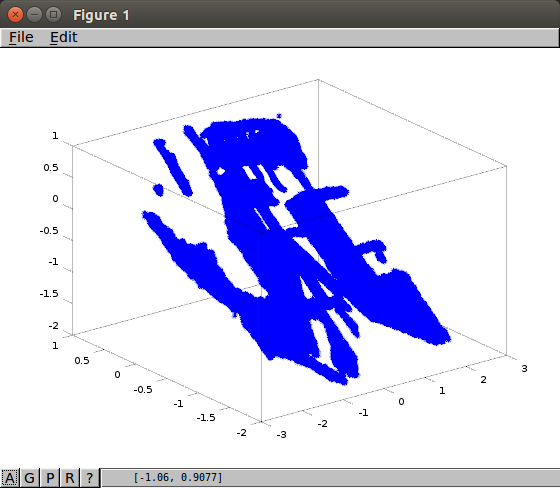
\includegraphics[width=.5\textwidth]{denseInitial}
    \caption{Exponential trend in KL distances.}
  \label{pcl:fig}
\end{figure}

The cloud is too dense to be correctly displayed in the plot. The planar components of the plane also dominate the cloud and its hard to operate on them. An image with a high amount of planar components is typical when data are acquired from a turtlebot with the camera being situated near the ground. In order to perform the clustering operations, the cloud needs to be downsampled. The process followed is the one described in the method definition and the results are shown in Fig~\ref{pcl:reduced}. The operation used is a pipeline voxel downsampling, statistical outlier removal and plane estimation via RANSAC is typical in the literature \cite{objectDisc}.


\begin{figure}[h!]
  \centering
    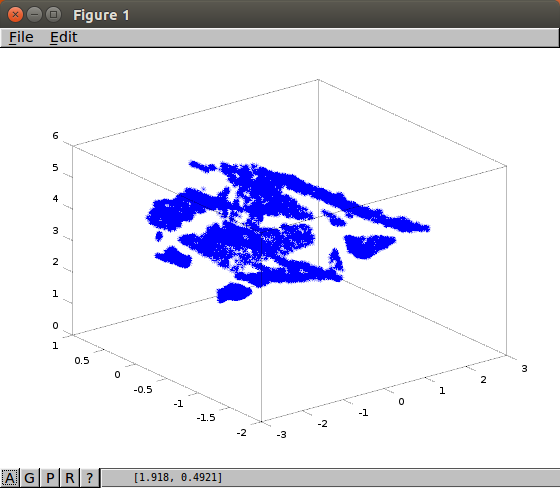
\includegraphics[width=.5\textwidth]{initial}
    \caption{Point cloud post pipeline modifications.}
  \label{pcl:reduced}
\end{figure}

The cloud is stripped of its planar components with the remaining structure having minimal to no loss of structural information. The cloud is now ready to be used as input for the sampler which will take the features calculated in the pipeline to cluster the cloud into segments of structure. The whole takes a medium amount of time and depending on the parameter tweaking it can 

The sampler as was described in the theory section takes as input the modified cloud and outputs clusters of the structure. Its results are shown in figure~\ref{pcl:clustering}. The environment is captured as a sequence of clusters. It can be seen that the chair that is situated in the center of the cloud has a number of clusters assigned to it. This behavior of the cluster is expected as a lot of point clouds are part of the chair and the horizontal as well and the vertical components have different angular signatures. It is not possible to create a general framework that takes into account all the different angle and point signatures between objects. The decision of how the clusters represent a structure should then be taken in a decision layer on top of that cluster. The random forest is build to classify objects by taking as input the output of the sampler.

\begin{figure}[h!]
  \centering
    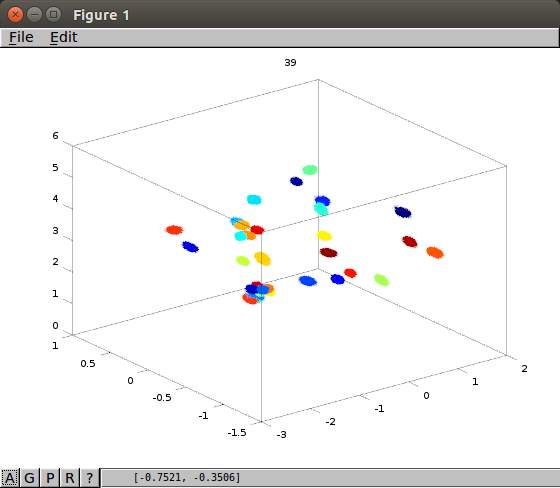
\includegraphics[width=.5\textwidth]{clustering}
    \caption{Point cloud post pipeline modifications.}
  \label{pcl:clustering}
\end{figure}

The random forest takes as input the distributions as given by the cluster and outputs the probability that each one represents an element the algorithm has previously already in the database. Only elements past a threshold will be considered as landmarks already encountered and otherwise the new distributions are added to the database. The features taken by the algorithm are the distances between each distribution and each landmark already stored in the database. More specifically, for the Gaussian parts of the distribution Wasserstein and Kullback Leibler divergence are used to measure the distance between them. For the exponential part, squared Hellinger and Kullback-Leibler being used, and for the categorical EMD, KL divergence and Hellinger distance. All distribution distances are given in the appendix. The final result is a 7 feature vector that will be used to classify if it's a distance signature that classifies a landmark or not. The training set is supplied beforehand to the algorithm. The results of the algorithm are shown in Fig.~\ref{pcl:features}

\begin{figure}[h!]
  \centering
    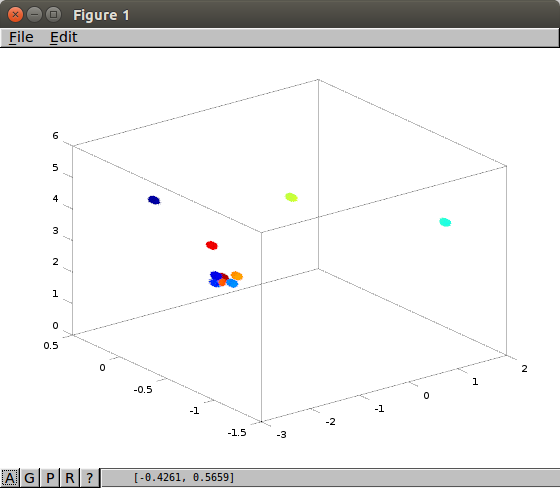
\includegraphics[width=.5\textwidth]{landmarkClasification}
    \caption{Point cloud post pipeline modifications.}
  \label{pcl:features}
\end{figure}

\section{Conclusion and future work}
\label{sec:discussion}

A novel method for SLAM by using compressed representations of objects in a point cloud is introduced. Its strengths and weaknesses are presented. Future work could include:
\begin{itemize}
    \item Improved tracking by using IMRF
    \item Extend to dynamic environments
    \item Extend the representation used
\end{itemize}
%------------------------------------------------

\section{Discussion}


\begin{thebibliography}{9}

\bibitem{probRobs}
\newblock Thrun, S. (2002). Probabilistic robotics. Communications of the ACM, 45(3), 52-57.


\bibitem{ekf}
\newblock Bailey, T., Nieto, J., Guivant, J., Stevens, M., \& Nebot, E. (2006, October). Consistency of the EKF-SLAM algorithm. In Intelligent Robots and Systems, 2006 IEEE/RSJ International Conference on (pp. 3562-3568). IEEE.

\bibitem{graph}
\newblock Thrun, S., \& Montemerlo, M. (2006). The graph SLAM algorithm with applications to large-scale mapping of urban structures. The International Journal of Robotics Research, 25(5-6), 403-429.

\bibitem{Figueredo:2009dg}
Figueredo, A.J. and Wolf, P. S.A. (2009).
\newblock Assortative pairing and life history strategy - a cross-cultural
  study.
\newblock {\em Human Nature}, 20:317--330.

\bibitem{liflonglearning}
\newblock Thrun, S., \& Mitchell, T. M. (1995). Lifelong robot learning. The Biology and Technology of Intelligent Autonomous Agents, 165-196.

\bibitem{lifelongmaps}
\newblock Konolige, K., \& Bowman, J. (2009, October). Towards lifelong visual maps. In Intelligent Robots and Systems, 2009. IROS 2009. IEEE/RSJ International Conference on (pp. 1156-1163). IEEE.

\bibitem{aishalong}
\newblock Walcott, A. (2011). Long-term robot mapping in dynamic environments (Doctoral dissertation, Massachusetts Institute of Technology).

\bibitem{bayesianNon}
\newblock Hjort, N. L., Holmes, C., Müller, P., \& Walker, S. G. (Eds.). (2010). Bayesian nonparametrics (Vol. 28). Cambridge University Press.

\bibitem{dependent}
\newblock {MacEachern, S. N. (2000) Dependent dirichlet processes. Unpublished manuscript, Department of Statistics, The Ohio State University.}

\bibitem{brml}
\newblock{Barber, D. (2012) Bayesian reasoning and machine learning.}

\bibitem{dependentDiri}
\newblock{Neiswanger, W., Wood, F., \& Xing, E.The dependent dirichlet process mixture of objects for detection-free tracking and object modeling. In Proceedings of the Seventeenth International Conference on Artificial Intelligence and Statistics (pp. 660-668) (2014, August) }

\bibitem{pcl}
\newblock{Rusu, R. B., \& Cousins, S. (2011, May). 3d is here: Point cloud library (pcl). In Robotics and Automation (ICRA), 2011 IEEE International Conference on (pp. 1-4). IEEE.}

\bibitem{rtabmap}
\newblock Labbé, M., \& Michaud, F. (2011, September). Memory management for real-time appearance-based loop closure detection. In Intelligent Robots and Systems (IROS), 2011 IEEE/RSJ International Conference on (pp. 1271-1276). IEEE.


\bibitem{slam++}
\newblock Salas-Moreno, R. F., Newcombe, R. A., Strasdat, H., Kelly, P. H., \& Davison, A. J. (2013, June). Slam++: Simultaneous localisation and mapping at the level of objects. In Computer Vision and Pattern Recognition (CVPR), 2013 IEEE Conference on (pp. 1352-1359). IEEE.

\bibitem{objslam}
\newblock Selvatici, A. H., \& Costa, A. H. (2008). Object-based visual slam: How object identity informs geometry.

\bibitem{castleetal}
\newblock Castle, R. O., Gawley, D. J., Klein, G., \& Murray, D. W. (2007, April). Towards simultaneous recognition, localization and mapping for hand-held and wearable cameras. In Robotics and Automation, 2007 IEEE International Conference on (pp. 4102-4107). IEEE.


\bibitem{objectpointslam}
\newblock Choudhary, S., Trevor, A. J., Christensen, H. I., \& Dellaert, F. (2014, September). SLAM with object discovery, modeling and mapping. In Intelligent Robots and Systems (IROS 2014), 2014 IEEE/RSJ International Conference on (pp. 1018-1025). IEEE.

\bibitem{objectpoint}
\newblock Jensfelt, P., Ekvall, S., Kragic, D., \& Aarno, D. (2006, September). Augmenting slam with object detection in a service robot framework. In Robot and Human Interactive Communication, 2006. ROMAN 2006. The 15th IEEE International Symposium on (pp. 741-746). IEEE.

\bibitem{monoslam}
\newblock Davison, A. J., Reid, I. D., Molton, N. D., \& Stasse, O. (2007). MonoSLAM: Real-time single camera SLAM. Pattern Analysis and Machine Intelligence, IEEE Transactions on, 29(6), 1052-1067.

\bibitem{objectDisc}
\newblock Koo, S., Lee, D., \& Kwon, D. S. (2014, September). Unsupervised object individuation from RGB-D image sequences. In Intelligent Robots and Systems (IROS 2014), 2014 IEEE/RSJ International Conference on (pp. 4450-4457). IEEE.


\bibitem{distMes}
\newblock{Cichocki, A., \& Amari, S. I.Families of alpha-beta-and gamma-divergences: Flexible and robust measures of similarities. Entropy, 12(6), 1532-1568.}

\bibitem{fpfh}
\newblock{Fast point feature histogram.Rusu, R. B., Blodow, N., \& Beetz, M. (2009, May). Fast point feature histograms (FPFH) for 3D registration. In Robotics and Automation, 2009. ICRA'09. IEEE International Conference on (pp. 3212-3217). IEEE.}

\bibitem{segOverview}
\newblock {Rabbani, T., van den Heuvel, F., \& Vosselmann, G. (2006). Segmentation of point clouds using smoothness constraint. International Archives of Photogrammetry, Remote Sensing and Spatial Information Sciences, 36(5), 248-253.}

\bibitem{gpu}
\newblock{Caron, F., Davy, M., \& Doucet, A. (2012) Generalized Polya urn for time-varying Dirichlet process mixtures. arXiv preprint arXiv:1206.5254.}


\bibitem{kinect}
\newblock{Zhang, Z. (2012) Microsoft kinect sensor and its effect. MultiMedia, IEEE, 19(2), 4-10.}

\bibitem{nonParam}
\newblock{Wainwright, M. J., \& Jordan, M. I. (2008). Graphical models, exponential families, and variational inference. Foundations and Trends in Machine Learning, 1(1-2), 1-305.}
``
\bibitem{omnimaper}
\newblock{A.Trevor,  J.Rogers, and  H.Christensen.  Omnimapper:  A  modular multimodal  mapping  framework.   In IEEE  International  Conference on Robotics and Automation (ICRA), 2014}

\bibitem{imft}
\newblock Koo, S., Lee, D., \& Kwon, D. S. (2013, November). Multiple object tracking using an rgb-d camera by hierarchical spatiotemporal data association. In Intelligent Robots and Systems (IROS), 2013 IEEE/RSJ International Conference on (pp. 1113-1118). IEEE.

\bibitem{pointSeg}
\newblock Trevor, A. J., Gedikli, S., Rusu, R. B., \& Christensen, H. I. (2013). Efficient organized point cloud segmentation with connected components. Semantic Perception Mapping and Exploration (SPME).

\bibitem{planarSeg}
\newblock Unnikrishnan, R., \& Hebert, M. (2003, October). Robust extraction of multiple structures from non-uniformly sampled data. In Intelligent Robots and Systems, 2003.(IROS 2003). Proceedings. 2003 IEEE/RSJ International Conference on (Vol. 2, pp. 1322-1329). IEEE. 

\bibitem{planarSeg2}
\newblock Rabbani, T., van den Heuvel, F., \& Vosselmann, G. (2006). Segmentation of point clouds using smoothness constraint. International Archives of Photogrammetry, Remote Sensing and Spatial Information Sciences, 36(5), 248-253.

\bibitem{smartSeg}
\newblock Triebel, R., Shin, J., \& Siegwart, R. (2010, June). Segmentation and unsupervised part-based discovery of repetitive objects. In Robotics: Science and Systems (Vol. 2).

\bibitem{smcddp}
\newblock Neiswanger, W., Wood, F., \& Xing, E. (2014, August). The dependent dirichlet process mixture of objects for detection-free tracking and object modeling. In Proceedings of the Seventeenth International Conference on Artificial Intelligence and Statistics (pp. 660-668).

\bibitem{corresp:first}
\newblock Cree, M. J., Jefferies, M. E., \& Baker, J. T. Using 3D Visual Landmarks to Solve the Correspondence Problem in Simultaneous Localisation and Mapping.

\bibitem{corres:sec}
\newblock Lowe, D. G. (2004). Distinctive image features from scale-invariant keypoints. International journal of computer vision, 60(2), 91-110.

\bibitem{corres:three}
\newblock Lamon, P., Tapus, A., Glauser, E., Tomatis, N., \& Siegwart, R. (2003, October). Environmental modeling with fingerprint sequences for topological global localization. In Intelligent Robots and Systems, 2003.(IROS 2003). Proceedings. 2003 IEEE/RSJ International Conference on (Vol. 4, pp. 3781-3786). IEEE.


\bibitem{corres:four}
\newblock Sehgal, A., Cernea, D., \& Makaveeva, M. (2010). Real-time scale invariant 3D range point cloud registration. In Image Analysis and Recognition (pp. 220-229). Springer Berlin Heidelberg.

\bibitem{bayes:neal}
\newblock Neal, R. M. (2000). Markov chain sampling methods for Dirichlet process mixture models. Journal of computational and graphical statistics, 9(2), 249-265.

\bibitem{bayes:jordan}
\newblock Blei, D. M., \& Jordan, M. I. (2006). Variational inference for Dirichlet process mixtures. Bayesian analysis, 1(1), 121-143.

\bibitem{slam}
\newblock{Montemerlo, M., Thrun, S., Koller, D., \& Wegbreit, B. (2002). FastSLAM: A factored solution to the simultaneous localization and mapping problem. AAAI/IAAI, 593-598.}

\bibitem{bayes:hier}
\newblock Teh, Y. W., Jordan, M. I., Beal, M. J., \& Blei, D. M. (2006). Hierarchical dirichlet processes. Journal of the american statistical association, 101(476).

\bibitem{bayes:smc}
\newblock Doucet, A., De Freitas, N., \& Gordon, N. (2001). An introduction to sequential Monte Carlo methods (pp. 3-14). Springer New York.

\bibitem{LDA}
\newblock{Blei, D. M., Ng, A. Y., \& Jordan, M. I. (2003). Latent dirichlet allocation. the Journal of machine Learning research, 3, 993-1022.}

\bibitem{theory:ddp}
\newblock MacEachern, S. N. (2000). -
\bibitem{speakerDiar}
f\newblock{Fox, E. B., Sudderth, E. B., Jordan, M. I., \& Willsky, A. S. (2011). A sticky HDP-HMM with application to speaker diarization. The Annals of Applied Statistics, 5(2A), 1020-1056.}


\bibitem{antoniak}
\newblock{Charles E Antoniak,Mixtures of dirichlet processes with applications to bayesian nonparametric problems, The annals of statistics (1974), 1152–1174}

\bibitem{caron}
\newblock{F. Caron, M. Davy, and A. Doucet, Generalized Polya urn for time-varying Dirichlet process mixtures, 23rd Conference on
Uncertainty in Artificial Intelligence (UAI’2007), Vancouver,
Canada, July 2007, 2007}

\bibitem{compendium}
\newblock{Fink, D. (1997). A compendium of conjugate priors.}

\bibitem{smc:theory}
\newblock{Ülker, Y., Günsel, B., \& Cemgil, A. T. (2010). Sequential Monte Carlo samplers for Dirichlet process mixtures. In International Conference on Artificial Intelligence and Statistics (pp. 876-883).}

\bibitem{doucet}
\newblock{Del Moral, P., Doucet, A., \& Jasra, A. (2006). Sequential monte carlo samplers. Journal of the Royal Statistical Society: Series B (Statistical Methodology), 68(3), 411-436.}

\bibitem{RANSAC}

\bibitem{conjugate}
\newblock Raiffa, H. (1974). Applied statistical decision theory.

\end{thebibliography}

%----------------------------------------------------------------------------------------



\end{document}